\chapter{Rut}


\section*{Introducción al Libro de Rut}

El \textbf{Libro de Rut} es el octavo libro del Antiguo Testamento y el tercero de los libros históricos. Es una narrativa breve pero profundamente significativa, centrada en la vida de Rut, una mujer moabita cuya fidelidad y determinación destacan en medio de la adversidad. El libro de Rut es único en el Antiguo Testamento por su énfasis en temas de lealtad, redención y la inclusión de extranjeros en el pueblo de Dios.

\subsection*{Autoría}

La autoría del libro de Rut es anónima, y su fecha de composición no está claramente definida. Algunos estudiosos sugieren que fue escrito durante la época del rey David o poco después, ya que conecta la historia de Rut con el linaje de David. Otros sostienen que fue compuesto durante el período del exilio babilónico, como un recordatorio de la importancia de la lealtad y la providencia divina.

\subsection*{Temática}

El libro de Rut aborda temas centrales de la fe y la humanidad, tales como:
\begin{itemize}
	\item \textbf{Lealtad y amor filial:} Rut decide permanecer junto a su suegra, Noemí, a pesar de las dificultades, mostrando un profundo compromiso.
	\item \textbf{Providencia divina:} La narrativa subraya cómo Dios obra a través de eventos cotidianos para cumplir sus planes redentores.
	\item \textbf{Redención:} La figura de Booz como pariente-redentor ilustra el concepto de redención en la cultura israelita, prefigurando la redención espiritual en el cristianismo.
	\item \textbf{Inclusión:} Rut, una moabita, se convierte en parte del pueblo de Israel, mostrando que la gracia de Dios trasciende las barreras étnicas.
\end{itemize}

\subsection*{Estructura Narrativa}

El libro de Rut tiene una estructura sencilla y cuidadosamente diseñada:
\begin{itemize}
	\item \textbf{Capítulo 1:} Rut y Noemí enfrentan la pérdida y regresan a Belén.
	\item \textbf{Capítulo 2:} Rut trabaja en los campos de Booz, donde comienza a surgir una relación.
	\item \textbf{Capítulo 3:} Rut se acerca a Booz para solicitar su redención.
	\item \textbf{Capítulo 4:} Booz redime a Rut y la toma como esposa, y se establece el linaje que conducirá a David.
\end{itemize}



El libro está ambientado en la época de los jueces, un período de inestabilidad política y religiosa en Israel. Sin embargo, su tono es marcadamente esperanzador, destacando la importancia de la fe y la bondad individual en medio de la incertidumbre. Además, sirve como un puente hacia la monarquía de David, conectando los eventos cotidianos con el plan divino para Israel.


El libro de Rut es una joya literaria y teológica que muestra cómo los actos de lealtad y bondad pueden tener un impacto eterno. Más allá de su importancia histórica, destaca la fidelidad de Dios y su capacidad para obrar a través de las vidas de personas comunes, llevando a cabo su plan redentor.


	\begin{center}
		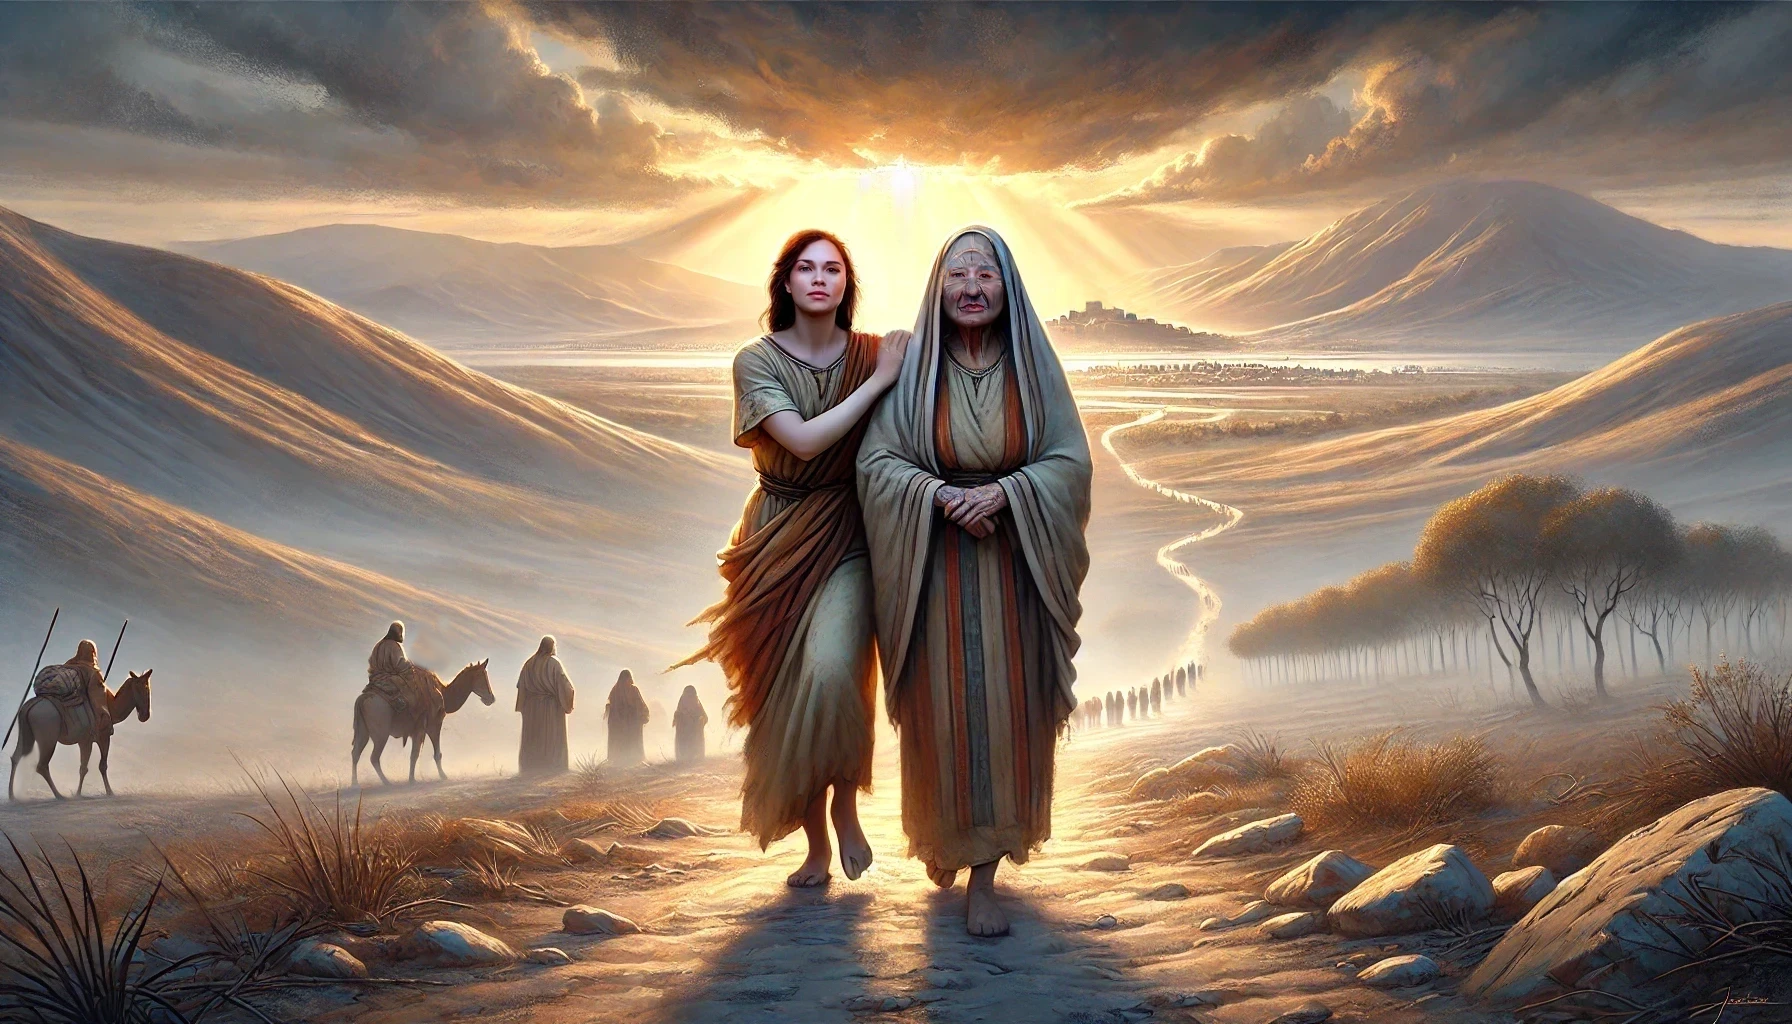
\includegraphics[width=0.7\linewidth]{graficas/Rut}\\
	Rut y Noemí  \\
	\end{center}



\section*{Capítulo 1}

Rut y Noemí  
1:1 Aconteció en los días que gobernaban los jueces, que hubo hambre en la tierra. Y un varón de Belén de Judá fue a morar en los campos de Moab, él y su mujer, y dos hijos suyos.  
1:2 El nombre de aquel varón era Elimelec, y el de su mujer, Noemí; y los nombres de sus hijos eran Mahlón y Quelión, efrateos de Belén de Judá. Llegaron, pues, a los campos de Moab, y se quedaron allí.  
1:3 Y murió Elimelec, marido de Noemí, y quedó ella con sus dos hijos,  
1:4 los cuales tomaron para sí mujeres moabitas; el nombre de una era Orfa, y el nombre de la otra, Rut; y habitaron allí unos diez años.  
1:5 Y murieron también los dos, Mahlón y Quelión, quedando así la mujer desamparada de sus dos hijos y de su marido.  
1:6 Entonces se levantó con sus nueras, y regresó de los campos de Moab; porque oyó en el campo de Moab que Jehová había visitado a su pueblo para darles pan.  
1:7 Salió, pues, del lugar donde había estado, y con ella sus dos nueras, y comenzaron a caminar para volverse a la tierra de Judá.  
1:8 Y Noemí dijo a sus dos nueras: Andad, volveos cada una a la casa de su madre; Jehová haga con vosotras misericordia, como la habéis hecho con los muertos y conmigo.  
1:9 Os conceda Jehová que halléis descanso, cada una en casa de su marido. Luego las besó, y ellas alzaron su voz y lloraron,  
1:10 y le dijeron: Ciertamente nosotras iremos contigo a tu pueblo.  
1:11 Y Noemí respondió: Volveos, hijas mías; ¿para qué habéis de ir conmigo? ¿Tengo yo más hijos en el vientre, que puedan ser vuestros maridos?  
1:12 Volveos, hijas mías, e idos; porque yo ya soy vieja para tener marido. Y aunque dijese: Esperanza tengo, y esta noche estuviese con marido, y aun diese a luz hijos,  
1:13 ¿habíais vosotras de esperarlos hasta que fuesen grandes? ¿Habíais de quedaros sin casar por amor a ellos? No, hijas mías; que mayor amargura tengo yo que vosotras, pues la mano de Jehová ha salido contra mí.  
1:14 Y ellas alzaron otra vez su voz y lloraron; y Orfa besó a su suegra, mas Rut se quedó con ella.  
1:15 Y Noemí dijo: He aquí tu cuñada se ha vuelto a su pueblo y a sus dioses; vuélvete tú tras ella.  
1:16 Respondió Rut: No me ruegues que te deje, y me aparte de ti; porque a dondequiera que tú fueres, iré yo, y dondequiera que vivieres, viviré. Tu pueblo será mi pueblo, y tu Dios mi Dios.  
1:17 Donde tú murieres, moriré yo, y allí seré sepultada; así me haga Jehová, y aun me añada, que sólo la muerte hará separación entre nosotras dos. 
1:18 Y viendo Noemí que estaba tan resuelta a ir con ella, no dijo más.  
1:19 Anduvieron, pues, ellas dos hasta que llegaron a Belén; y aconteció que habiendo entrado en Belén, toda la ciudad se conmovió por causa de ellas, y decían: ¿No es ésta Noemí?  
1:20 Y ella les respondía: No me llaméis Noemí, sino llamadme Mara; porque en grande amargura me ha puesto el Todopoderoso.  
1:21 Yo me fui llena, pero Jehová me ha vuelto con las manos vacías. ¿Por qué me llamaréis Noemí, ya que Jehová ha dado testimonio contra mí, y el Todopoderoso me ha afligido?  
1:22 Así volvió Noemí, y Rut la moabita su nuera con ella; volvió de los campos de Moab, y llegaron a Belén al comienzo de la siega de la cebada.  
\section*{Capítulo 2}
Rut recoge espigas en el campo de Booz  

2:1 Tenía Noemí un pariente de su marido, hombre rico de la familia de Elimelec, el cual se llamaba Booz.  
2:2 Y Rut la moabita dijo a Noemí: Te ruego que me dejes ir al campo, y recogeré espigas en pos de aquel a cuyos ojos hallare gracia. Y ella le respondió: Vé, hija mía.  
2:3 Fue, pues, y llegando, espigó en el campo en pos de los segadores; y aconteció que aquella parte del campo era de Booz, el cual era de la familia de Elimelec.  
2:4 Y he aquí que Booz vino de Belén, y dijo a los segadores: Jehová sea con vosotros. Y ellos respondieron: Jehová te bendiga.  
2:5 Y Booz dijo a su criado el mayordomo de los segadores: ¿De quién es esta joven?  
2:6 Y el criado, mayordomo de los segadores, respondió y dijo: Es la joven moabita que volvió con Noemí de los campos de Moab;  
2:7 y ha dicho: Te ruego que me dejes recoger y juntar tras los segadores entre las gavillas. Entró, pues, y está desde por la mañana hasta ahora, sin descansar ni aun por un momento.  
2:8 Entonces Booz dijo a Rut: Oye, hija mía, no vayas a espigar a otro campo, ni pases de aquí; y aquí estarás junto a mis criadas.  
2:9 Mira bien el campo que sieguen, y síguelas; porque yo he mandado a los criados que no te molesten. Y cuando tengas sed, ve a las vasijas, y bebe del agua que sacan los criados.  
2:10 Ella entonces bajando su rostro se inclinó a tierra, y le dijo: ¿Por qué he hallado gracia en tus ojos para que me reconozcas, siendo yo extranjera?  
2:11 Y respondiendo Booz, le dijo: He sabido todo lo que has hecho con tu suegra después de la muerte de tu marido, y que dejando a tu padre y a tu madre y la tierra donde naciste, has venido a un pueblo que no conociste antes.  
2:12 Jehová recompense tu obra, y tu remuneración sea cumplida de parte de Jehová Dios de Israel, bajo cuyas alas has venido a refugiarte.  
2:13 Y ella dijo: Señor mío, halle yo gracia delante de tus ojos; porque me has consolado, y porque has hablado al corazón de tu sierva, aunque no soy ni como una de tus criadas.  
2:14 Y Booz le dijo a la hora de comer: Ven aquí, y come del pan, y moja tu bocado en el vinagre. Y ella se sentó junto a los segadores, y él le dio del potaje, y comió hasta que se sació, y le sobró.  
2:15 Luego se levantó para espigar. Y Booz mandó a sus criados, diciendo: Que recoja también espigas entre las gavillas, y no la avergoncéis;  
2:16 y dejaréis también caer para ella algo de los manojos, y lo dejaréis para que lo recoja, y no la reprendáis.  
2:17 Espigó, pues, en el campo hasta la noche, y desgranó lo que había recogido, y fue como un efa  de cebada.  
2:18 Y lo tomó, y se fue a la ciudad; y su suegra vio lo que había recogido. Sacó también luego lo que le había sobrado después de haber quedado saciada, y se lo dio.  
2:19 Y le dijo su suegra: ¿Dónde has espigado hoy? ¿y dónde has trabajado? Bendito sea el que te ha reconocido. Y contó ella a su suegra con quién había trabajado, y dijo: El nombre del varón con quien hoy he trabajado es Booz.  
2:20 Y dijo Noemí a su nuera: Sea él bendito de Jehová, pues que no ha rehusado a los vivos la benevolencia que tuvo para con los que han muerto. Después le dijo Noemí: Nuestro pariente es aquel varón, y uno de los que pueden redimirnos.  
2:21 Y Rut la moabita dijo: Además de esto me ha dicho: Júntate con mis criadas, hasta que hayan acabado toda mi siega.  
2:22 Y Noemí respondió a Rut su nuera: Mejor es, hija mía, que salgas con sus criadas, y que no te encuentren en otro campo.  
2:23 Estuvo, pues, junto con las criadas de Booz espigando, hasta que se acabó la siega de la cebada y la del trigo; y vivía con su suegra.  
\section*{Capítulo 3}
Rut y Booz en la era  

3:1 Después le dijo su suegra Noemí: Hija mía, ¿no he de buscar hogar para ti, para que te vaya bien?  
3:2 ¿No es Booz nuestro pariente, con cuyas criadas tú has estado? He aquí que él avienta esta noche la parva de las cebadas.  
3:3 Te lavarás, pues, y te ungirás, y vistiéndote tus vestidos, irás a la era; mas no te darás a conocer al varón hasta que él haya acabado de comer y de beber.  
3:4 Y cuando él se acueste, notarás el lugar donde se acuesta, e irás y descubrirás sus pies, y te acostarás allí; y él te dirá lo que hayas de hacer.  
3:5 Y ella respondió: Haré todo lo que tú me mandes.  
3:6 Descendió, pues, a la era, e hizo todo lo que su suegra le había mandado.  
3:7 Y cuando Booz hubo comido y bebido, y su corazón estuvo contento, se retiró a dormir a un lado del montón. Entonces ella vino calladamente, y le descubrió los pies y se acostó.  
3:8 Y aconteció que a la medianoche se estremeció aquel hombre, y se volvió; y he aquí, una mujer estaba acostada a sus pies.  
3:9 Entonces él dijo: ¿Quién eres? Y ella respondió: Yo soy Rut tu sierva; extiende el borde de tu capa sobre tu sierva, por cuanto eres pariente cercano.  
3:10 Y él dijo: Bendita seas tú de Jehová, hija mía; has hecho mejor tu postrera bondad que la primera, no yendo en busca de los jóvenes, sean pobres o ricos.  
3:11 Ahora pues, no temas, hija mía; yo haré contigo lo que tú digas, pues toda la gente de mi pueblo sabe que eres mujer virtuosa.  
3:12 Y ahora, aunque es cierto que yo soy pariente cercano, con todo eso hay pariente más cercano que yo.  
3:13 Pasa aquí la noche, y cuando sea de día, si él te redimiere, bien, redímate; mas si él no te quisiere redimir, yo te redimiré, vive Jehová. Descansa, pues, hasta la mañana.  
3:14 Y después que durmió a sus pies hasta la mañana, se levantó antes que los hombres pudieran reconocerse unos a otros; porque él dijo: No se sepa que vino mujer a la era.  
3:15 Después le dijo: Quítate el manto que traes sobre ti, y tenlo. Y teniéndolo ella, él midió seis medidas  de cebada, y se las puso encima; y ella se fue a la ciudad.  
3:16 Y cuando llegó a donde estaba su suegra, ésta le dijo: ¿Qué hay, hija mía? Y le contó ella todo lo que con aquel varón le había acontecido.  
3:17 Y dijo: Estas seis medidas  de cebada me dio, diciéndome: A fin de que no vayas a tu suegra con las manos vacías.  
3:18 Entonces Noemí dijo: Espérate, hija mía, hasta que sepas cómo se resuelve el asunto; porque aquel hombre no descansará hasta que concluya el asunto hoy.  
\section*{Capítulo 4}
Booz se casa con Rut  

4:1 Booz subió a la puerta y se sentó allí; y he aquí pasaba aquel pariente de quien Booz había hablado, y le dijo: Eh, fulano, ven acá y siéntate. Y él vino y se sentó.  
4:2 Entonces él tomó a diez varones de los ancianos de la ciudad, y dijo: Sentaos aquí. Y ellos se sentaron.  
4:3 Luego dijo al pariente: Noemí, que ha vuelto del campo de Moab, vende una parte de las tierras que tuvo nuestro hermano Elimelec.  
4:4 Y yo decidí hacértelo saber, y decirte que la compres en presencia de los que están aquí sentados, y de los ancianos de mi pueblo. Si tú quieres redimir, redime; y si no quieres redimir, decláramelo para que yo lo sepa; porque no hay otro que redima sino tú, y yo después de ti. Y él respondió: Yo redimiré.  
4:5 Entonces replicó Booz: El mismo día que compres las tierras de mano de Noemí, debes tomar también a Rut la moabita, mujer del difunto, para que restaures el nombre del muerto sobre su posesión.  
4:6 Y respondió el pariente: No puedo redimir para mí, no sea que dañe mi heredad. Redime tú, usando de mi derecho, porque yo no podré redimir.  
4:7 Había ya desde hacía tiempo esta costumbre en Israel tocante a la redención y al contrato, que para la confirmación de cualquier negocio, el uno se quitaba el zapato y lo daba a su compañero; y esto servía de testimonio en Israel.  
4:8 Entonces el pariente dijo a Booz: Tómalo tú. Y se quitó el zapato. 
4:9 Y Booz dijo a los ancianos y a todo el pueblo: Vosotros sois testigos hoy, de que he adquirido de mano de Noemí todo lo que fue de Elimelec, y todo lo que fue de Quelión y de Mahlón.  
4:10 Y que también tomo por mi mujer a Rut la moabita, mujer de Mahlón, para restaurar el nombre del difunto sobre su heredad, para que el nombre del muerto no se borre de entre sus hermanos y de la puerta de su lugar. Vosotros sois testigos hoy.  
4:11 Y dijeron todos los del pueblo que estaban a la puerta con los ancianos: Testigos somos. Jehová haga a la mujer que entra en tu casa como a Raquel y a Lea, las cuales edificaron la casa de Israel; y tú seas ilustre en Efrata, y seas de renombre en Belén.  
4:12 Y sea tu casa como la casa de Fares, el que Tamar dio a luz a Judá, por la descendencia que de esa joven te dé Jehová.  
4:13 Booz, pues, tomó a Rut, y ella fue su mujer; y se llegó a ella, y Jehová le dio que concibiese y diese a luz un hijo.  
4:14 Y las mujeres decían a Noemí: Loado sea Jehová, que hizo que no te faltase hoy pariente, cuyo nombre será celebrado en Israel;  
4:15 el cual será restaurador de tu alma, y sustentará tu vejez; pues tu nuera, que te ama, lo ha dado a luz; y ella es de más valor para ti que siete hijos.  
4:16 Y tomando Noemí el hijo, lo puso en su regazo, y fue su aya.  
4:17 Y le dieron nombre las vecinas, diciendo: Le ha nacido un hijo a Noemí; y lo llamaron Obed. Este es padre de Isaí, padre de David.  
4:18 Estas son las generaciones de Fares: Fares engendró a Hezrón,  
4:19 Hezrón engendró a Ram, y Ram engendró a Aminadab,  
4:20 Aminadab engendró a Naasón, y Naasón engendró a Salmón,  
4:21 Salmón engendró a Booz, y Booz engendró a Obed,  
4:22 Obed engendró a Isaí, e Isaí engendró a David.
